\documentclass[UTF8]{ctexart}

\usepackage{graphicx}
\usepackage{amsmath}
\usepackage{float}

\title{DoubleLikedList}

\author{林敬翊 \\ 信息与计算科学 \\ 3210300367}

\date{2022年10月6日}

\begin{document}

\maketitle

\begin{abstract}

双向链表也叫双链表,是链表的一种,它的每个数据结点中都有两个指针,分别指向直接后继和直接前驱。所以,从双向链表中的任意一个结点开始,都可以很方便地访问它的前驱结点和后继结点。一般我们都构造双向循环链表。\\

\textbf{关键词}:双链表

\end{abstract}

\section{设计}

在我的程序设计里面 我采用了switch option的选项自己选择自己想要的形式输入,然后里面的功能主要有6种,分别是正常添加Node,在首位添加新的Node,在特定的节点位后添加node,删除node,更新node和print。


\section{添加Node}
在添加Node里面,一共有三种添加方法。\\
第一种是正常添加,也就是他会自动植入在最后一个位置,如果没有最后一个,他就会放在第一个,以此类推。\\
第二种是添加在首位,也就是会自动植入在第一个位置,如果没有任何数据,将自动植入在第一个,以此类推。\\
第三种是添加在特定的点位。首先先选定特定的点位,然后将Node添加在此点位之后。

\section{更新和删除Node算法}
更新node:输入你要改的程序的编号,然后输入他的key 和 data。\\
删除node: 输入你要删除的程序的编号,然后他就会删除了。

\section{print}
最后最后就是print list了,只要有东西他就会print出来,没有的话会返回 `没有Node在DoublyLinkedList里面'

\begin{figure}[H]
  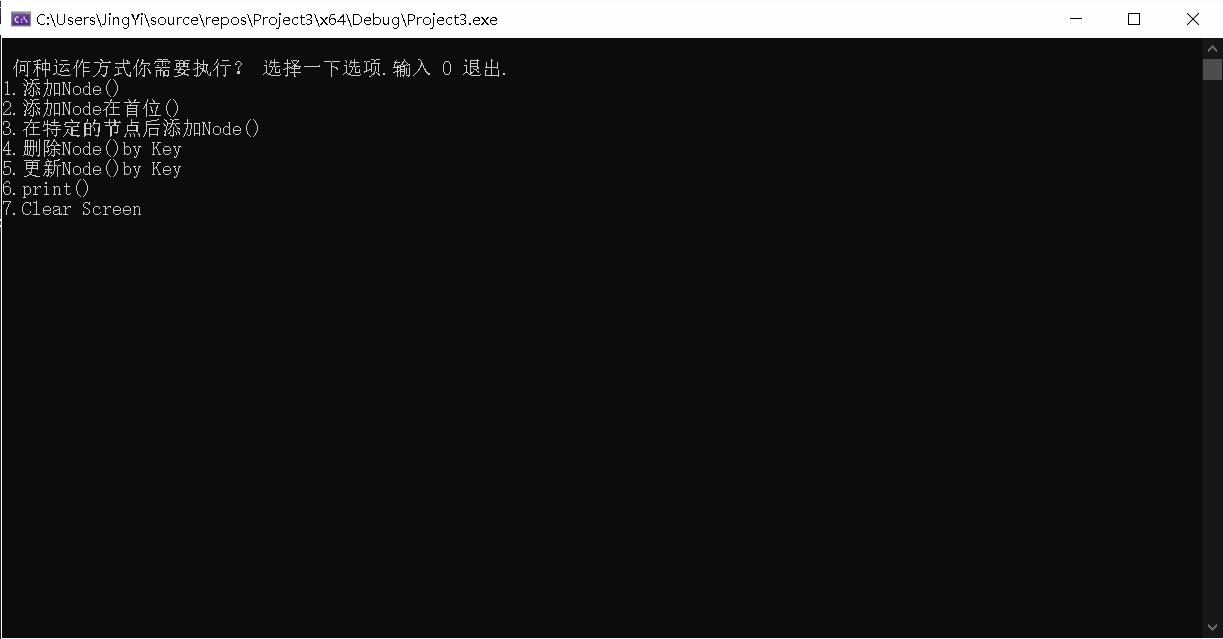
\includegraphics[width=\linewidth]{123.jpg}
  \centering
  \caption{程序开始}
\end{figure}

\end{document}
